\documentclass[a4paper,11pt]{report}
\usepackage[utf8]{inputenc}
\usepackage{amsmath}
\usepackage[T1]{fontenc}
\usepackage{graphicx}
\usepackage{wrapfig}
\usepackage{caption}
\usepackage{enumitem}
\usepackage{pdfpages}
\usepackage{multicol}
\usepackage[a4paper, left=3cm, right=3cm, top=3cm, bottom=3cm]{geometry}
\usepackage[ngerman]{babel}
\usepackage{hyperref}
\usepackage[dvipsnames]{xcolor}
\usepackage{fancyhdr}
\pagestyle{fancy}

% set font

% hyperlink setup
\hypersetup{
    colorlinks,
    citecolor=black,
    filecolor=black,
    linkcolor=Emerald,
    urlcolor=black
}

% clear Footer
\fancyfoot{}

% Header
\fancyhead[L]{Andrin Tim Lerjen, \\ Nadja Rahm, Niklas Fister}
\fancyhead[C]{Kantonnschule - Physik}
\fancyhead[R]{\thepage}
\renewcommand{\headrulewidth}{1pt}

\fancypagestyle{plain}{
    \fancyhead[L]{Andrin Tim Lerjen, \\ Nadja Rahm, Niklas Fister}
    \fancyhead[C]{Kantonnschule - Physik}
    \fancyhead[R]{\thepage}
    \renewcommand{\headrulewidth}{1pt}
}

% Title
\title{\Huge\textbf{Bericht Physik - Lautsprecher}}
\author{Andrin Tim Lerjen, Nadja Rahm, Niklas Fister}
\date{\today}

% makeing title
\begin{document}
\pagenumbering{Roman}
\maketitle

% Abstract
\newpage
\begin{abstract}
    In dem Folgenden Bericht geht es um die Bau eines Lautsprechers aus alltäglichen Materialien.

    Es wurde ein Leistungsstarken Lautsprecher gebaut, was vor allem an den starken Magneten liegt.

    Die Bauart aus leichten Materialien für den Schallerzeuger und dem stabilen Klangkörper sorgen für ein gutes Klangerlebnis.
    
\end{abstract}

% Table of contents
\newpage
\tableofcontents
\thispagestyle{empty}

% report
\newpage
\pagenumbering{arabic}
\setcounter{page}{1}

% Bericht
\part{Bericht}

% Introduction
\chapter{Einleitung}
\section{Fragestellung}
\begin{enumerate}
    \item Ist es möglich in der Schule einen gut funktionierenden Lautsprecher zu bauen?
    \item Ist es sinvoller einen Magneten innerhalb der Spule oder ausserhalb zu positionieren?
    \item Empfiehlt sich ein dickerer oder dünnerer Draht?
\end{enumerate}
\section{Hypothese}
\begin{enumerate}
    \item Wir gehen davon aus, dass wir einen Lautsprecher bauen können, der bei mittleren Lautstärken funktioniert, aber Schwächen bei sehr lauten Tönen und Bässen hat.
    \item Wir gehen davon aus, dass es sinvoller ist den Magneten ausserhalb der Spule zu positionieren.
    \item Wir gehen davon aus, dass ein dicker Draht sinvoller ist, da er weinger Widerstand hat und somit weniger Wärme erzeugt.
\end{enumerate}

\newpage
\section{Theorie}
\subsection{Wichtige Formeln}
\textbf{Relevante Variablen} \\
\(\mu_0\) : magnetische Permeabilität des Vakuums \\
\(\mu_r\) : magnetische Permeabilität des Füllmaterials \\
\(N\) : Anzahl Windungen \\
\(I\) : Stromstärke \\
\(L\) : Länge der Spule \\

\textbf{Berechnung der magnetischen Permeabilit im Vakuum}
\begin{equation}
    \mu_0 = 4 \cdot \pi \cdot 10^{-7} \frac{V \cdot s}{A \cdot m}
\end{equation}

\textbf{Berechnung der magnetischen Kraft mit Füllmaterial}
\begin{equation}
    B(r) \approx \frac{\mu_0 \cdot \mu_r \cdot N \cdot I}{L}
\end{equation}

\subsection{Geschichte des Lautsprechers}

\begin{wrapfigure}{r}{0.4\textwidth}
    \centering
    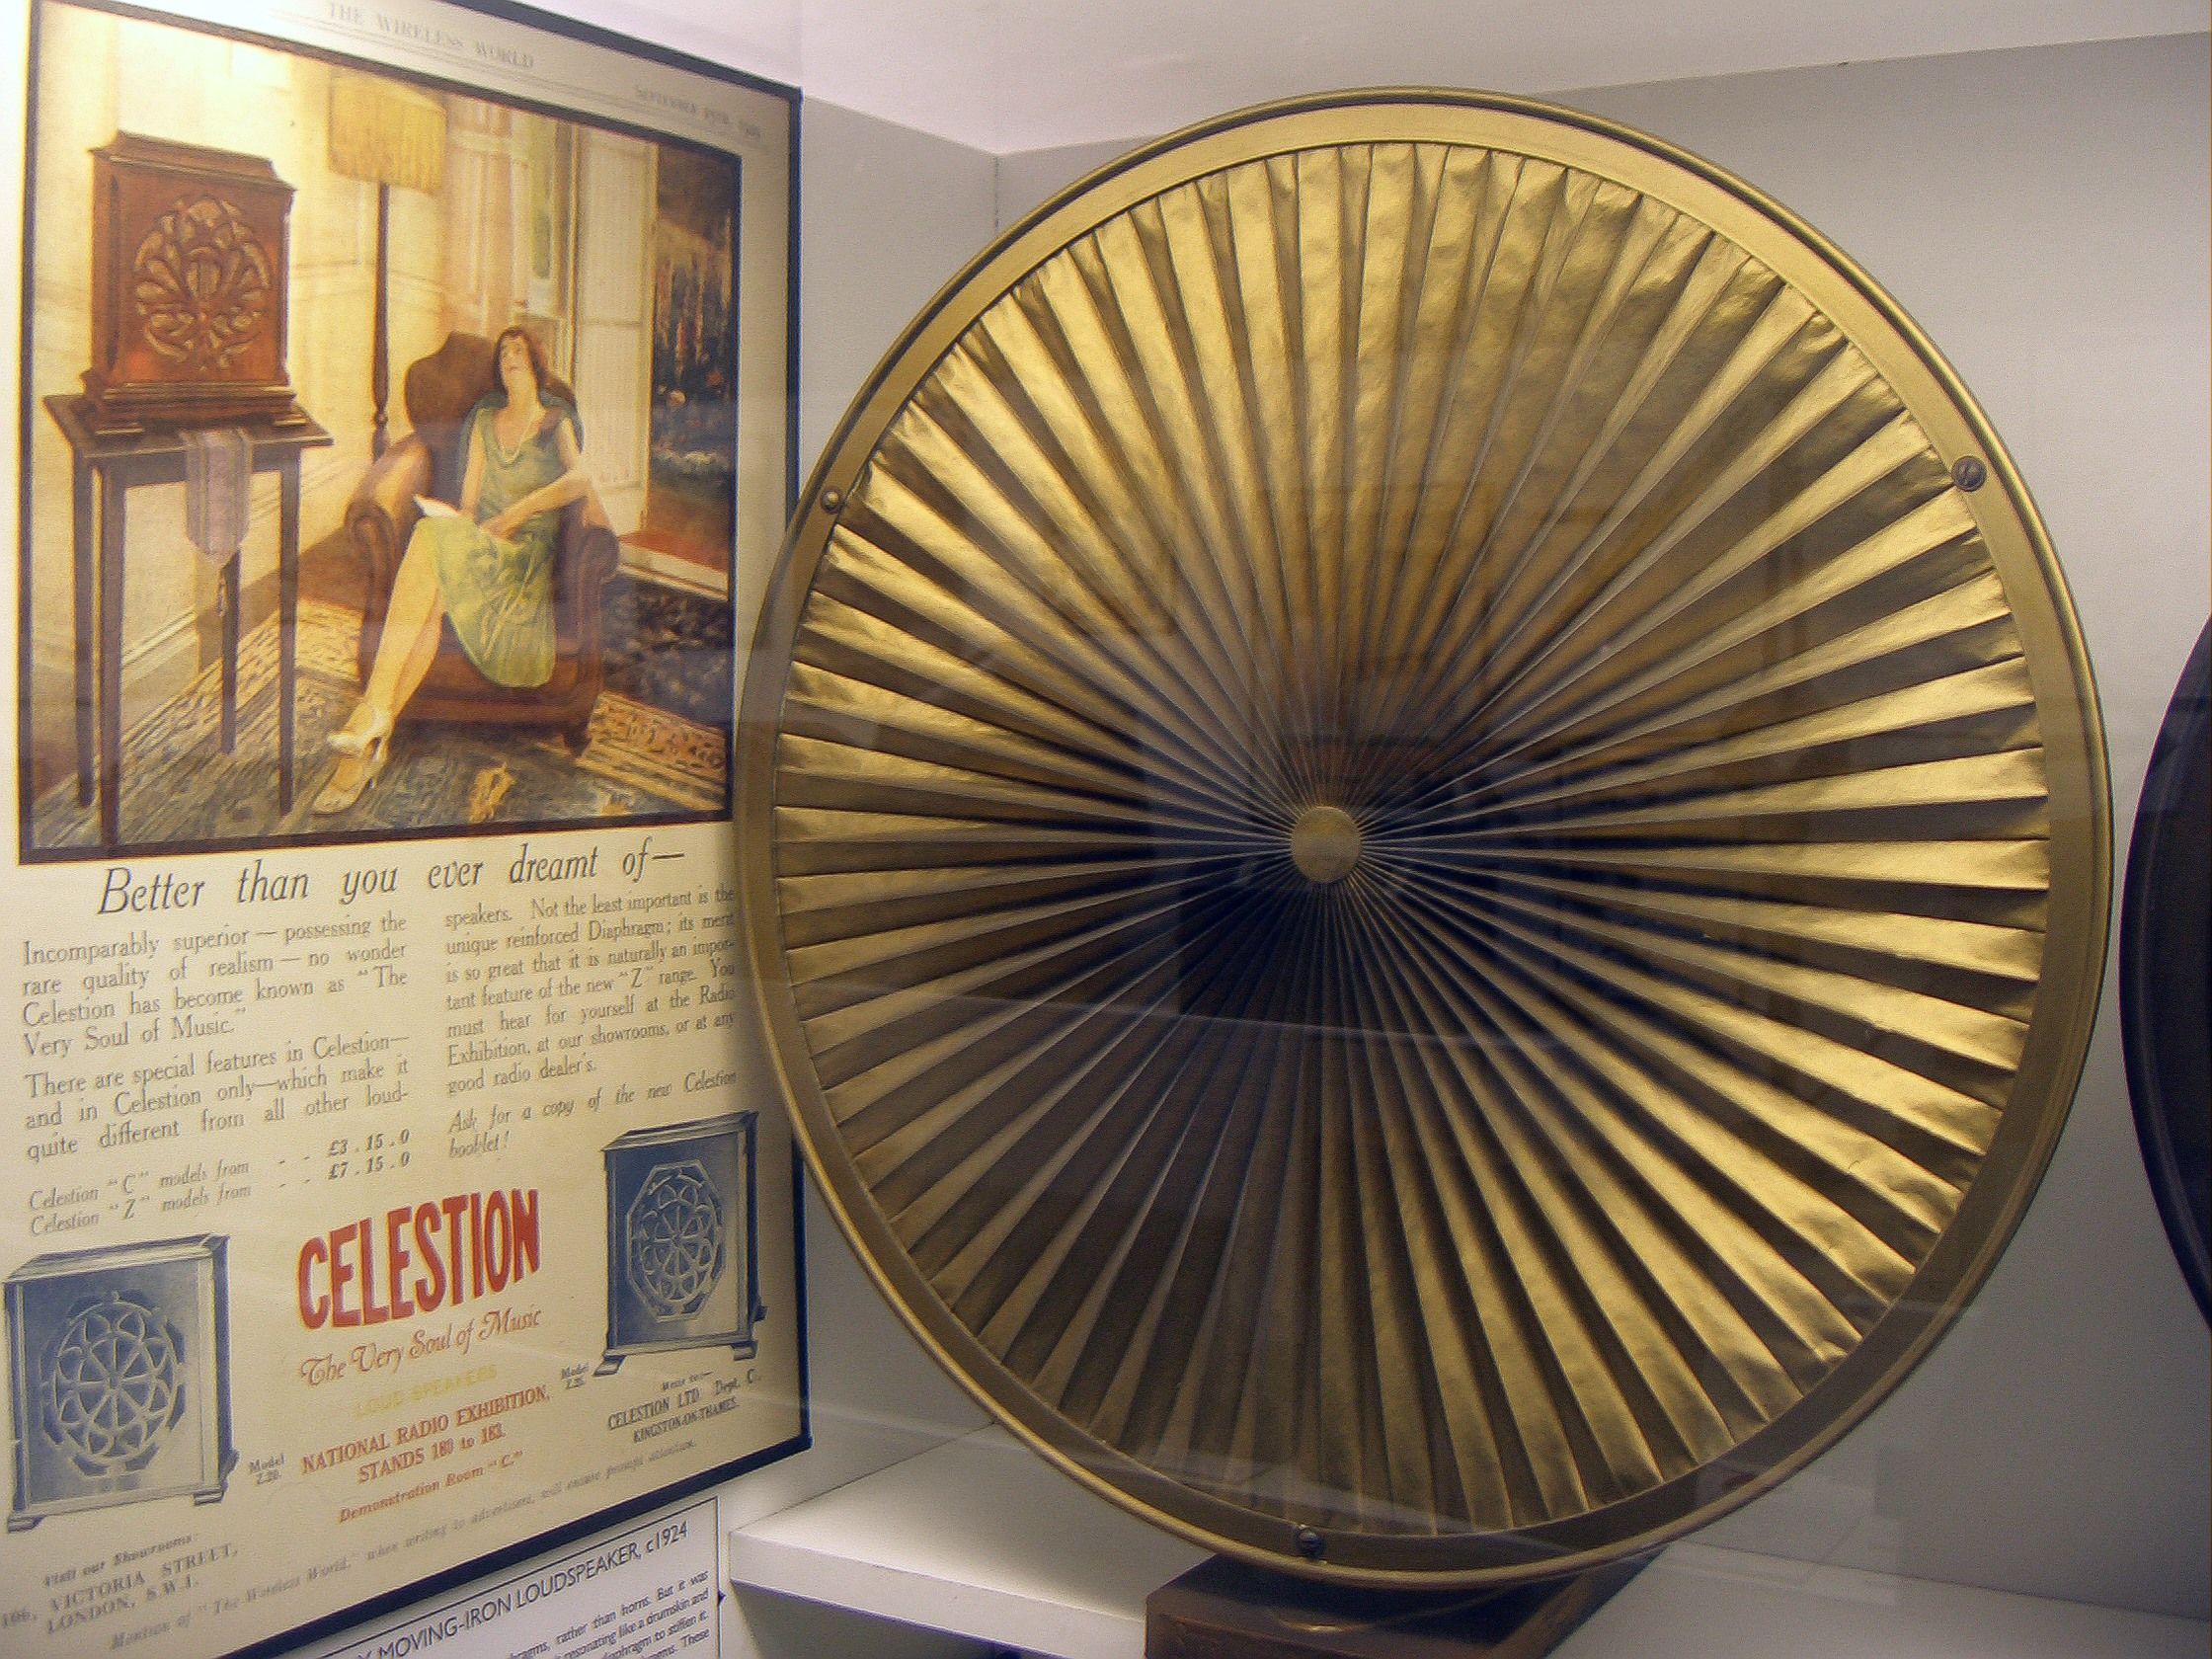
\includegraphics[width=.95\linewidth]{resources/images/Lautsprecher_Celestion.jpg}
    \caption{Lautsprecher von Celestion}
    \label{fig:celection_speaker}
\end{wrapfigure}

Der Lautsprecher wurde im Jahre 1861 als mechanisches Nebenprodukt des Telefons entwickelt.

1878 wurde dann das Patent zu einem elektrischen Lautsprecher eingereicht, welches letztlich erst 1925 präsentiert wurde.
Das Grundprinzip blieb bis heute unverändert und ist in den Meisten Lautsprechern Vorzufinden. \cite{history_wikipedia}

Aufgrund der damaligen Bauart waren die Lautsprecher meinst sehr gross. Dies war Aufgrund der weichen Einspannung. \cite{history_connect}

Einen Entwickler für den Lautsprecher kann man jedoch nicht genau nennen, da es eine fliessende Entwicklung war, welche zum dem Produkt führten.

Vielen forschten gleichzeitig in diesem Thema und Patente unterschieden sich nur wage. Teils waren die Patente in den USA und Deutschland sogar nahezu identisch.\cite{history_tu_berlin}

% How to build it properly
\subsection{Ideale Bauweise}

\begin{wrapfigure}{r}{0.2\textwidth}
    \centering
    \includegraphics[width=.95\linewidth]{resources/images/Bassreflex-Gehäuse.png}
    \caption{Bassreflex-Gehäuse}
    \label{fig:bassreflex}
\end{wrapfigure}

Um eine möglichst guten Bass zu generieren ist die Bauart eines Bassreflex-Gehäuses optimal. Durch die offene Bauweise mit einem sogenannten "Bassrefelexkanal" versehen.
Das Innere des Körpers wird als Resonator gebraucht, um den Bass zu verstärken.

Dabei wird als allgemeine Formel für die Berechnung der Resonator-Kanälen mit kreisförmigen Querschnitt:\\
d : Durchmesser (in cm) \\
l : Länge (in cm)

\begin{equation}
    l = \frac{23400 \cdot d^2}{f^2 \cdot V_b} - 0.8 \cdot d
\end{equation}
\cite{bassreflex_wikipedia}

% Materials and Methods
\chapter{Material und Methoden}
\section{Material}
\begin{multicols}{2}
    \begin{itemize}[parsep=0pt]
        \item Schleifpapier (für Klangerzeuger und Kupferdraht zu endisolieren)
        \item Kupferdraht (0.5mm)
        \item Kupferdraht (0.4mm)
        \item Karton für den Körper der Spule
        \item Bananenkabel
        \item Isolierband (gelb)
        \item Zähler (für Umwicklungen)
        \item Verstärker
        \item Kartonbox
        \item Schere
        \item Cutter
        \item Multimeter
        \item Taschenmesser
    \end{itemize}
\end{multicols}
\section{Methoden}
\section{Bauplan}
\chapter{Resultate}
\chapter{Diskussion}

% Baudokumentation
\part{Baudokumentation}

% How to build it
\chapter{Plan}

% How it was built
\chapter{Bau}

% List of figures
\newpage
\listoffigures

% Sources
\newpage
\bibliographystyle{plain}
\bibliography{mybib}
\end{document}